\documentclass[a4paper,12pt]{article}
\usepackage{graphicx}
\usepackage{eso-pic}
\usepackage[utf8]{inputenc}
\usepackage[T1]{fontenc}
\usepackage[french]{babel}

\usepackage[colorlinks=True,citecolor=black,urlcolor=blue,linkcolor=black]{hyperref}
\usepackage{subfigure}
\usepackage[francais]{layout}
\usepackage{color}
\usepackage[table]{xcolor}
\usepackage{listings}
\usepackage{fancyhdr}
\lstset{
aboveskip=3mm,
belowskip=-2mm,
backgroundcolor=\color{darkWhite},
basicstyle=\footnotesize,
breakatwhitespace=false,
breaklines=true,
captionpos=b,
commentstyle=\color{red},
deletekeywords={...},
escapeinside={\%*}{*)},
extendedchars=true,
framexleftmargin=16pt,
framextopmargin=3pt,
framexbottommargin=6pt,
frame=tb,
keepspaces=true,
keywordstyle=\color{blue},
language=C,morekeywords={*,...},
numbers=left,
numbersep=10pt,
numberstyle=\tiny\color{black},
rulecolor=\color{black},
showspaces=false,
showstringspaces=false,
showtabs=false,
stepnumber=1,
stringstyle=\color{gray},
tabsize=4,
title=\lstname,
}


\usepackage[utf8]{inputenc}
\title{Projet jeu Darkest Dungeon}
\author{\textsc{Monjoux} Hugo & \textsc{Rivière} Hadrien & Option IS TP1}
\date{27 Septembre 2018}
\usepackage[a4paper,top=1.5cm,bottom=1.5cm,left=1.5cm,right=1.5cm,marginparwidth=1.75cm]{geometry}

\pagestyle{fancy}
\fancyhf{}
\chead{MONJOUX Hugo | RIVIERE Hadrien | Rendu 1.1 | Page \thepage}

\begin{document}
\maketitle
\begin{figure}[!ht]
  \centering
  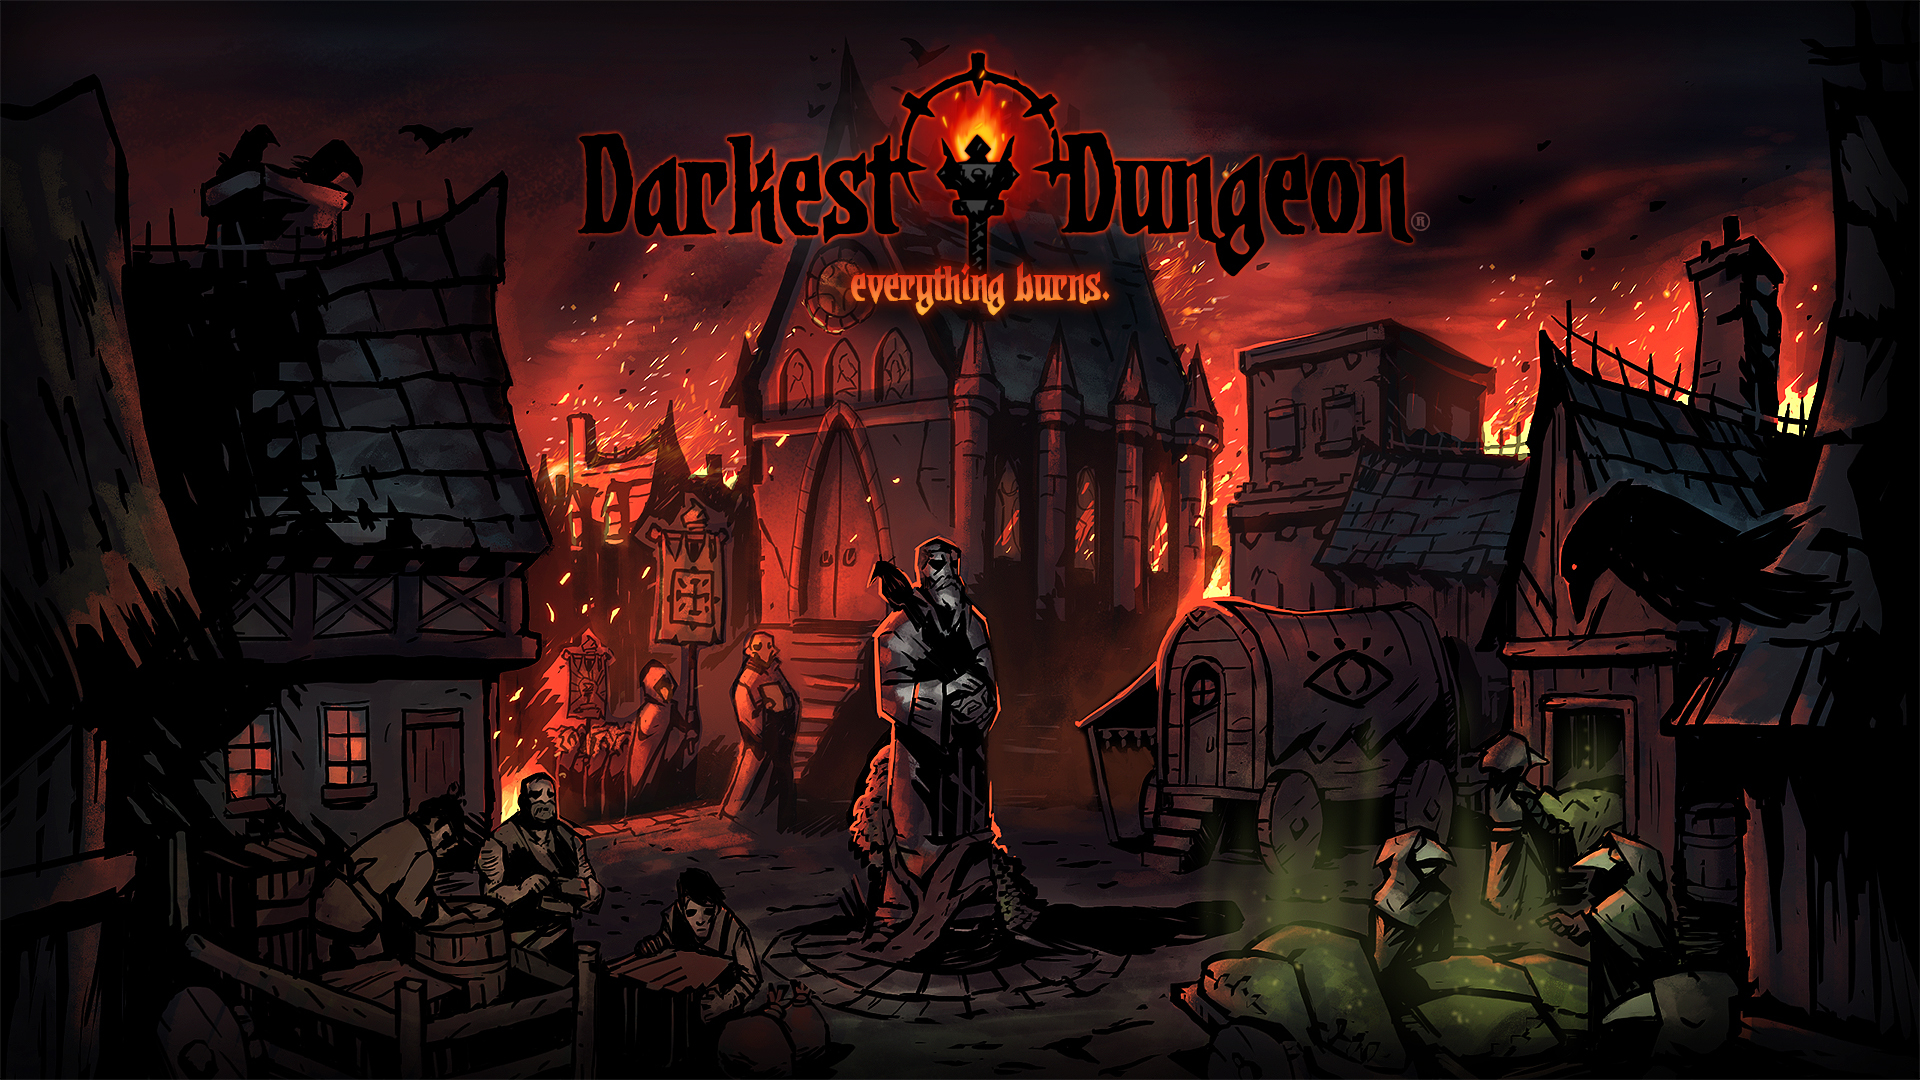
\includegraphics[width=1\textwidth]{Rendu1/ecran_acceuil.jpg}
  \caption{Aperçu du jeu "The Darkest Dungeon"}
\end{figure}

\newpage
\tableofcontents
\newpage
\section{Présentation Générale}
\subsection{Archétype}
Notre jeu s'inspire de Darkest Dungeon, qui est un RPG tour par tour, Rogue-like. Ce jeu est illustré dans les différentes figures exposées en fin du rapport. 

\subsection{Règles du jeu}

 Ce dernier permet au joueur d'évoluer soit en tant que héros, soit en tant qu'ennemis. L'objectif du joueur varie donc selon ce choix fait en début de partie. Si le joueur choisit de jouer en tant que héros, il doit arriver à la fin du niveau. Dans l'autre cas le joueur doit s'assurer que les héros n'arrive pas à la fin du niveau. 
\\ 
\indent
Le jeu se compose en trois vues : 
\begin{itemize}
    \item Vue d'accueil du joueur, qui pourra définir son équipe de héros, ainsi que l'inventaire de l'équipe, soit la répartition des ennemis sur les cartes de jeu
    \item Vue de déplacement dans le donjon
    \item Vue de combat lors de la confrontation des héros avec les ennemis
\end{itemize} 
\subsection{Ressources}
\begin{figure}[!ht]
  \centering
  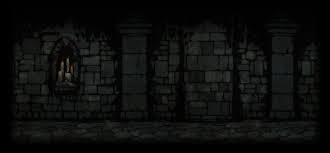
\includegraphics[width=0.8\textwidth]{Rendu1/background3.jpg}
  \caption{Premier élément de décor : couloir}
\end{figure}
\begin{figure}[!ht]
  \centering
  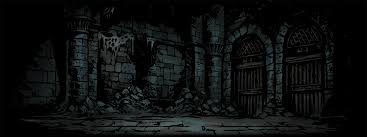
\includegraphics[width=0.8\textwidth]{Rendu1/background4.jpg}
  \caption{Deuxième élément de décor : salle}
\end{figure}
\begin{figure}[!ht]
  \centering
  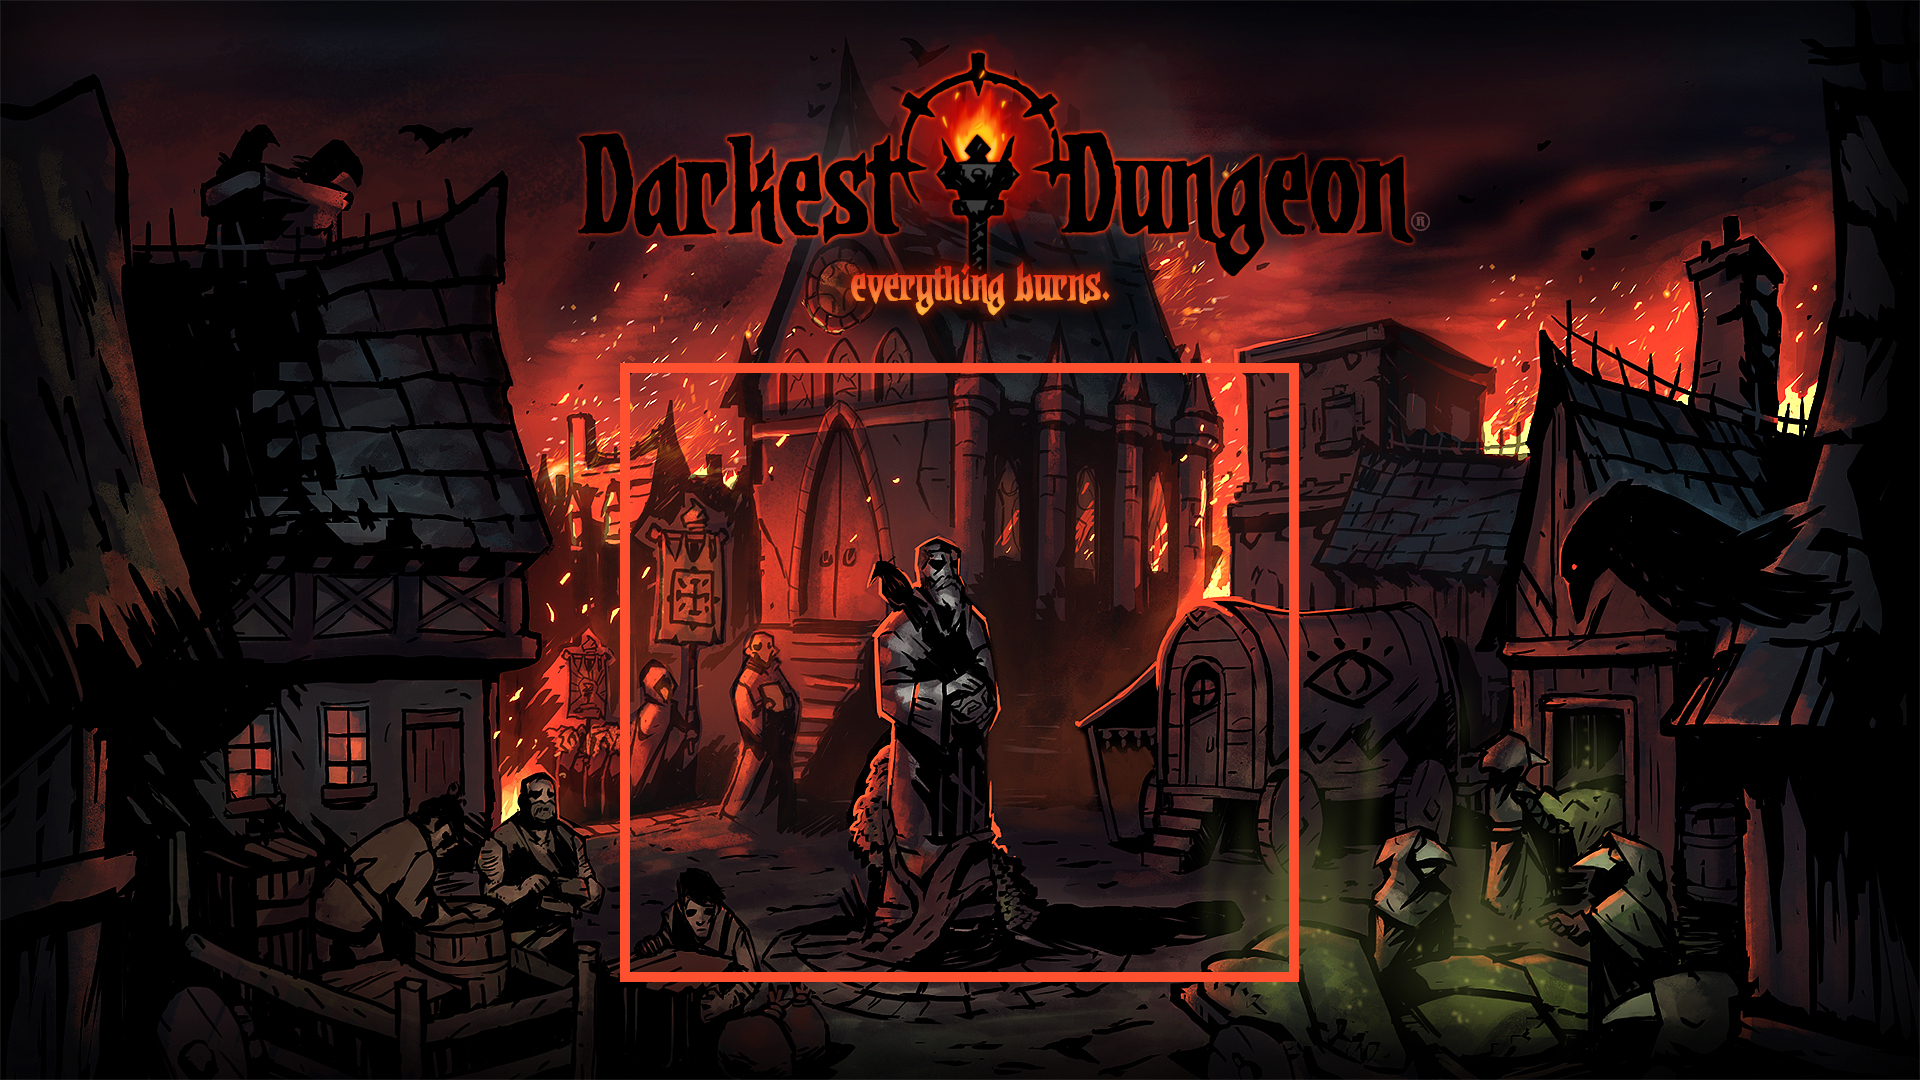
\includegraphics[width=1\textwidth]{Rendu1/ecran_acceuil.png}
  \caption{Ecran d'accueil avec à l'intérieur du cadre, le menu d'accueil (New game, Options...)}
\end{figure}
\begin{figure}[!ht]
  \centering
  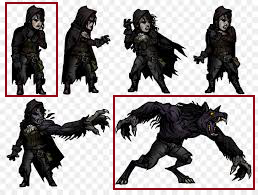
\includegraphics[width=0.6\textwidth]{Rendu1/pers_licantrope.png}
  \caption{Exemple de design d'un personnage se transformant. Seulement les sprites encadrés seront utilisés pour alléger les ressources.}
\end{figure}
\begin{figure}[!ht]
  \centering
  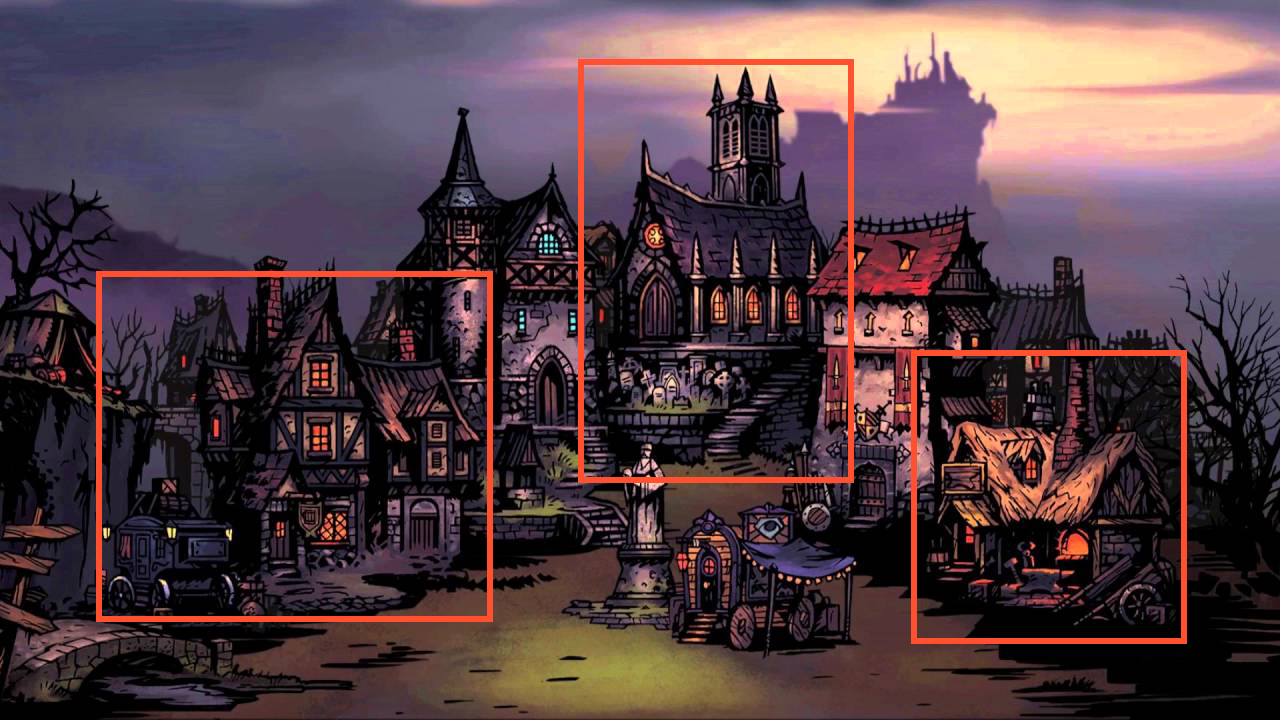
\includegraphics[width=1\textwidth]{Rendu1/city1.png}
  \caption{Ville d'accueil du joueur avec de gauche à droite encadrés :  Auberge de recrutement pour modifier l'équipe, Sauvegarde de la progression, et Magasin pour remplir l'inventaire de l'équipe.}
\end{figure}
\begin{figure}[!ht]
  \centering
  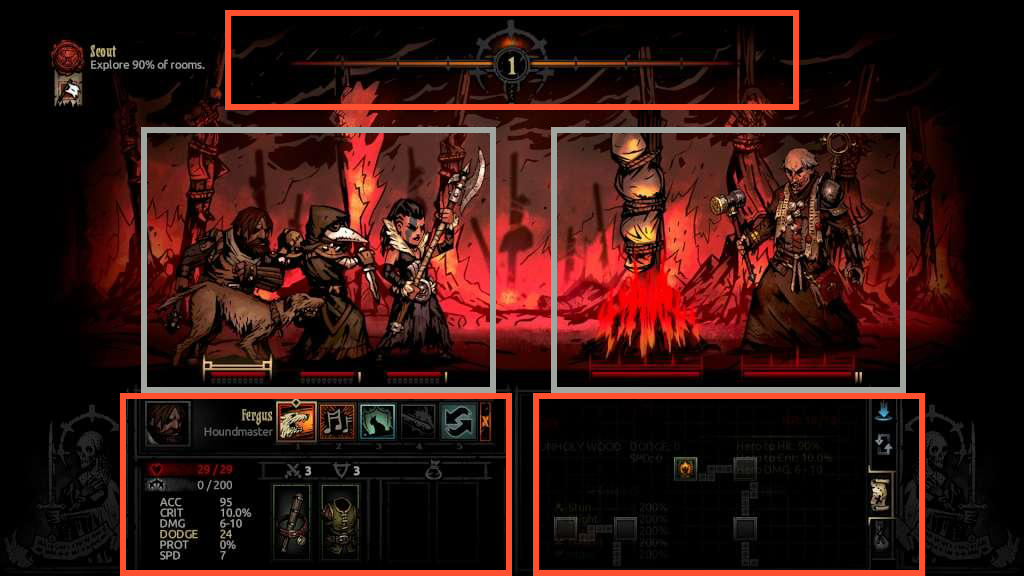
\includegraphics[width=1\textwidth]{Rendu1/combat.png}
  \caption{Ecran de jeu principal : encadrés en gris clair, les héros à gauche et les ennemis à droite avec leur barre de vie respectives situées en dessous | encadrés en orange, les différents outils à dispositions du joueur (compétences, statistiques des personnages, équipements, carte, inventaire). Ces éléments seront adaptés aux contraintes de temps et de moyens de notre projet.}
\end{figure}





\end{document}